\section{Introduction}
\label{sec-introduction}

% introduce LPL asynchronous duty cycle media access
As already we are aware, smartphones have become a necessity in our lives, as we are checking our mobile phones constantly throughout the day. As a result, some privacy concerns have arisen about nearby parties peeking at our screen, namely ``shoulder surfing". 
Assuming that the attacker is not malicious and merely takes several peeks out of curiosity, most works in this area are built on a threat model of an attacker observing with naked eyes. And studies show that a great portion of these attacks are casual and opportunistic without technical equipment~\cite{eiband2017understanding}, say a mere stranger can hardly do any harm reading a fragment of the correspondence or acquiring the password without knowing the account for critical apps like Alipay, which seldom appears on screen in common usages. 
% It is however the rare but malicious attacker, with certain familiarity and knowledge of the victim, that can do the most harm. The attacker can even be our closest friends or family members, as there are various cases in China where a child obtains Alipay password of their parents and is unaware that electronic payments consists of 'real' money, resulting in spending them lavishly in their games. Besides, specially designed equipment are not a necessity for the shoulder surfing attack. 

The privacy threat however has been exacerbated with smartphones improved significantly these years. Given the commercial smartphone, the attacker can not only reduce suspicion by acquiring sensitive information from a long distance, but also record the information for propagating, rendering greater damage to the victim. For example, in a Senate hearing, the Justice Secretary of Philippines, Vitaliano Aguirre II, suffered a leakage of his text messages, as someone had taken a snapshot of his smartphone \cite{Polotiko2017leakage}.Equipped with multiple cameras, the newest generation of smartphones can perform 100$\times$ zooming compared to the standard 5$\times$ of single camera phones. Hardware improvements in memory also allows the burst mode at tremendous frame rates and even high-speed photography, delivering videos with thousands of frames per second. And more images means more recorded information of the victim. To gain vital data stealthily from even further away, the processing technique of multi-frame super resolution (SR) algorithms can be employed by the attacker, delivering a more threatening shoulder surfing model.

% In this present era where the leakage of a password and the disclosure of correspondence of public figures can cause great damage to the victim, we believe that it's imminent to recall attention on this new privacy threat and propose the corresponding standard of screen protection based on modern circumstances.

To mitigate this threat, massive efforts have been made, from physical privacy films to alternative password entry interfaces \cite{wiedenbeck2006design,papadopoulos2017illusionpin} and input methods \cite{kumar2007reducing}. All of these methods however require additional cost and/or effort \cite{Chun2019Keep} and are not widely deployed yet on the critical privacy stages (e.g., password entry) of most everyday apps. And none of existing work can deal with the presence of smartphone cameras and SR algorithms in shoulder surfing scenarios. Given that the leakage of a password and the disclosure of correspondence of public figures can cause great damage to the victim, we believe that it's imminent to recall attention on this new privacy threat and propose the corresponding standard of screen protection based on modern circumstances.

\cl{The challenge part can be revised to make it more precise. And it can be described with the new figure.}
\vspace{1mm}
\noindent
\textbf{challenges.} Creating a high-resolution shoulder surfing attack model running on commercial smartphones in real time, however, is not trivial. And we achieve \textsf{SRPeek} by overcoming three key challenges.

\begin{itemize}[leftmargin=*]
  \item \textbf{Blurriness of input images.} The most prominent one is the blurriness, as our photos are taken at extreme range, taken secretly and hurriedly without much room for focusing, while straining the magnification of the smartphone lenses. Unlike most SR applications and datasets working with ‘normally’ captured photos, the images we face exhibit lower concentrations of information and more artifacts, and needs more ‘reconstruction’ than ‘interpolation’.
  \item \textbf{Processing with multi-frames.} While exploring this privacy threat, we need a multi-frame SR algorithm on a smartphone to monitor the target phone in real time. However, we discover that there is no existing SR algorithm suitable for this scenario. On one hand, images captured by hand are blurred while most methods rely on a handful of clearer images (e.g., scenery, scanned images) \cite{nasrollahi2020deep,lyn2020image}. Specifically, we have to extract the information from large quantities of extremely blurred photos, as smartphones can capture 100 snapshots in a few seconds in burst mode, and these photos are taken from extreme distances. On the other hand, the difference between videos and multiple snapshots rules out the video super resolution algorithms, which cannot be adapted to larger numbers of input images. The reason has two folds. First, either increased input leads to increases in model complexity, making it unsuitable for mobile deployment. Second, they lack an emphasis on the process of horizontal comparison(??) by relying heavily on the information extracted from each single image, resulting in an inefficient merge of information from multiple frames.
  \item \textbf{Compatibility with various characters.} Another difficulty unique to our task is the subject—mainly, Chinese characters. Composed of multiple strokes, these characters are distributed discretely in image space, not known to other entities, e.g. faces and natural objects. In some cases, messing up a stroke will not impact its readability, and in other cases shortening or lengthening a stroke even slightly will lead to a different character, leading to misunderstandings. And unlike most SR applications working on similarity (between their output and the ‘ground truth’), our goal is readability, and the network architecture and training process must be engineered accordingly.
\end{itemize}
 
\begin{figure}
	\centering
	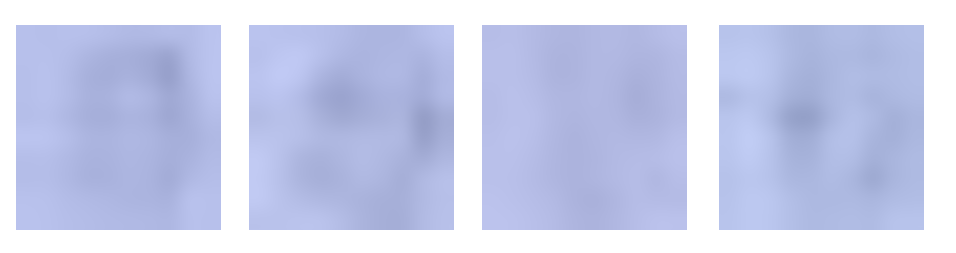
\includegraphics[width=0.48\textwidth]{pic/zeros.png}
    \caption{Photos of number ‘0’ on a screen at a distance of 1.5m, taken in quick succession from a still smartphone camera. All exhibit different blurriness and no consistency between neighboring frames.\cl{Figure should be replaced.}}
	\label{fig-zeros}
\end{figure}

\cl{The following part can correspond to challenges above.}
In this paper, we present \textsf{SRPeek}, an end-to-end system of shoulder surfing for commercial smartphones. To fully explore this privacy threat with the multi-frame super resolution, we first design a deep learning architecture using convolutional neural network (CNN). With the specially designed network as core, we deliver a holistic system for shoulder surfing on a smartphone. Then it processes them with our neural network to generate a high-resolution image and repeats the process for constant monitoring. As the information of interest is mostly in the form of text (e.g., passwords or e-mails), our network is trained and evaluated on the task of reconstructing text, specifically, Chinese characters, English letters, and numbers, but we believe that this network architecture can function in all scenarios. Our system can also be used as a preprocessor for text-recognition applications when multiple images are available, such as real-time translation apps on a smartphone or text-recognition on self-driving cars.

To deal with massive frames of blurred images with limited computational resources on smartphones, we design an unique merging layer and place it between convolutional layers in the SR pipeline. Thus information can be extracted first from input images independently and then merged together, serving as a reference for the following convolutions.

As mentioned above, reconstructing images with high degrees of blurriness requires a unique approach. Most works on multi-frame SR function on video clips \cite{lucas2019generative} or multiple snapshots \cite{wronski2019handheld}, however, our application is subtly different from the two. Our dilemma is as follows: on one hand, each one of the photos we are to process is blurred with a randomly different PSF kernel, which, because of the extreme blurriness, cannot be approximated as a constant, isotropic gaussian kernel, and thus lacking consistency between neighboring frames, meaning that they cannot be processed as a video clip(see Figure~\ref{fig-zeros} ); on the other hand, because of the low concentration of information, the blurred photos are similar to pieces of a jigsaw puzzle, each containing only fractions of information, and the only chance of recovering the ground truth is by comparing each photo against others. If processed by common procedures enhancing the resolution of a series of snapshots—processing each one separately and merging them afterwards, few useful information can be extracted from each one of the images, and merging them will not produce satisfactory results.

Considering the unique challenges of our application, we believe that if these images are processed iteratively, alternating between the following two processes, our network will be able to solve this ‘jigsaw puzzle’:

\begin{enumerate}
  \item Every single image of the input collection will be processed solely (by several layers of CNN), with access of the output of step (2) of the last iteration;
  \item The processed results will be merged (with weighted averaging methods) and distributed to each photo for the next iteration.
\end{enumerate}

This architecture is beneficial to our task. On one hand, the deep learning part is assigned to each single image, reducing computational complexity and parameter growth, while receiving a global view of all the images, renewed at each layer, thanks to the merging process; on the other hand, information can be shared horizontally with weighted averaging methods, meaning no consideration of sequential order and no reliance of consistency between neighboring frames. Thus, this architecture solves the dilemma mentioned above, and proves perfectly functional in our application.

\vspace{1mm}
\noindent
\textbf{Contributions.} This paper makes the following contributions:
\begin{itemize}[leftmargin=*]
  \item	We propose \textsf{SRPeek}, a multi-frame SR neural network architecture aiming at reconstructing extremely blurred and defocused images. This model is not only functional in our scenario, as a shoulder-surfing threat model, but also can be used in text-recognition applications prior to recognition algorithms to increase accuracy.
  \item	We design a threat model of shoulder-surfing, with the attacker armed with multi-frame SR algorithms and taking multiple photos (in burst mode) of the victim’s screen with a smartphone camera. To the best of our knowledge, we are the first to consider the presence of smartphone cameras and SR algorithms in shoulder surfing scenarios.
  \item	We demonstrate the effect of this shoulder-surfing attack and prove that it poses a threat to screen privacy.
\end{itemize}

% describe the organization of the paper
The rest of the paper is organized as follows. Section 2 describes the threat model of our  carefully studies the performance of state-of-the-art concurrent flooding. The detailed design of COFlood protocol is shown in Section~\ref{sec-design}. We show the implementation details and evaluation results in Section~\ref{sec-implementation-and-evaluation}. The related work is introduced in Section~\ref{sec-related-work}. Finally, we conclude our work in Section~\ref{sec-conclusion}.
